% this file is called up by thesis.tex
% content in this file will be fed into the main document

\chapter{Evaluation}\label{ch:evaluation} % top level followed by section, subsection


% ----------------------- paths to graphics ------------------------

% change according to folder and file names
\ifpdf
    \graphicspath{{figures/PNG}}
\else
    \graphicspath{{7/figures/EPS/}{7/figures/}}
\fi


% ----------------------- contents from here ------------------------
% 
In this section, the experiment results are presented.
The RDMA transportation types are compared within and against the baseline TCP implementation.
Throughput and latency are mainly used to analysis the scalability of these transportation types.
Both measurements are taken from the same run TODO WHICH WORDING?, annd corresponds? can be used interchanbly?

In short, the results show:
\begin{itemize}
    \item Throughput scales with all transportation types up to 30 clients. UD performs best, with a TODO ADD PERCENTAGE increase per client. Further details are given in section \ref{sec:throughput-analysis}.
    \item Latency increases across all transportation types. Results are inversly comparable to throughput, again with UD performing best. Section \ref{sec:latency:analysis} delves deeper.
\end{itemize}

To recall the benchmarking setup:
Ten million tasks are divided equally between \textit{n}-clients.
A task is defined as a request and response, and are equal to two operations.

\section{Throughput analysis}\label{sec:throughput-analysis}
We compare the average throughput between TCP, RC, and UD with up to 30 clients.
It is to be expected that CPU dependent TCP will perform poorly, with RDMA performing significantly better.
Connection oriented transportation types will scale similarly with each other, however connectionless should scale better.

\begin{figure}
    \centering
    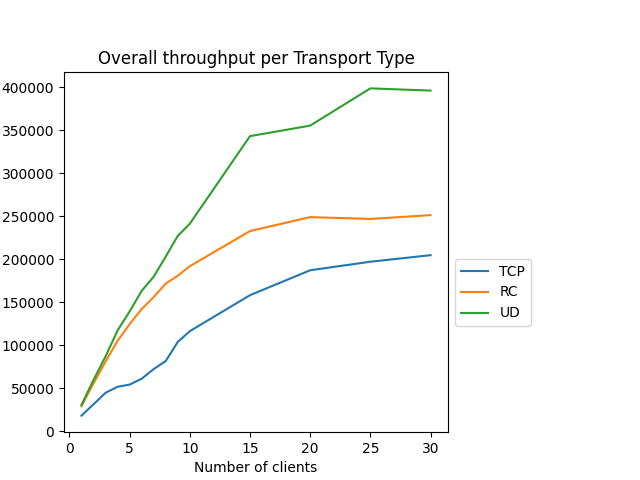
\includegraphics[height=80mm]{/home/jtroo/Documents/VU/Thesis/RDMA-KV-store/benchmarking/graphs/Throughput_30}
    \caption{Throughput of clients executing 10 million operations}
    \label{fig:throughput-30}
\end{figure}

\subsection{Scalability rate}\label{subsec:scalability-rate}
It can be observed from figure \ref{fig:throughput-30} that all transportation types scale up to roughly 20 clients before settling.
UD outperforms the other types, in both throughput and rate of scalability.
UD reaches a maximum of 398 kilo tasks/sec.
A near linear scalability rate can be seen in the first 15 clients for UD.
This is due the addition of threads for every new client.
Since all these threads are actively working for all clients, this linear increase is to be expected.
For the first 10 clients, UD increases its throughput by 23.4 kilo tasks/sec per additional client.
Compare this with 18.1 for RC and 10.9 kilo tasks/sec for the baseline TCP.
This shows strong scalability for UD with small number of clients.
It is unclear from this graph if UD continues to scale beyond 30 clients.

\subsection{Similarities between RC and TCP}
It can also be seen in figure \ref{fig:throughput-30} that RC is similar to TCP in scalability.
With both being a connection oriented protocol, each server thread being tied to a client, it shows similar performance.
The benefits of RDMA do reflect in these results, with the throughput of RC being on average 59.7 Ktasks/sec above TCP.

\subsection{Fairness between clients}
TODO GENERATE GRAPH FOR THIS

\section{Latency analysis}\label{sec:latency:analysis}
An important factor to KV store is their quick response time, and therefore this should ideally scale similarly, preferably better, than throughput.
RDMA offers fast response time due to the lack of CPU and kernel involvement.
To see how this is translated per transportation type, the average latency of all 10 million tasks were measured, from request sent to response received.
Results can be seen in figure \ref{fig:latency-30}.
Along with the average latency, the first and third quartile are shown, to analyze the variation of latencies.

\begin{figure}
    \centering
    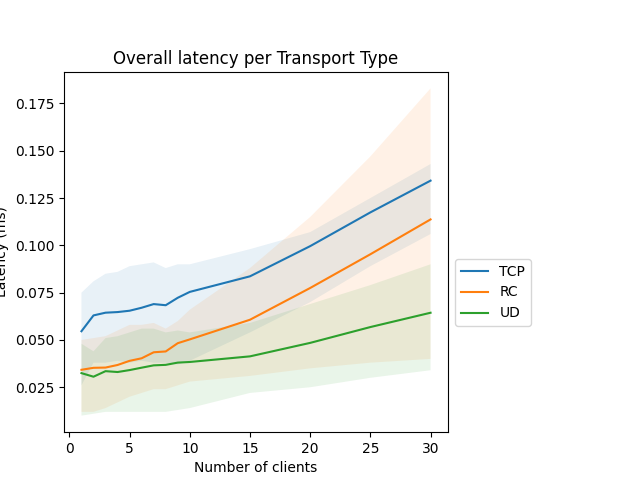
\includegraphics[height=80mm]{figures/PNG/Latency_avg_30}
    \caption{Latency of clients executing 10 million operations}
    \label{fig:latency-30}
\end{figure}

\subsection{Overall observations that can be made}
The latency between protocols is an inverse reflection of the throughput graph, scaling and overall performance.
Similarly, TCP performed worst, with an average latency of 0.135ms TODO ACCURATE NUMBER at 30 clients.
RC following the same path as TCP and hits an average of 0.11ms, also at 30 clients.
UD again performing best, reaching 0.06ms on average.

Similarly to throughput, UD scales relatively well.
A near uniform latency for the first 15 clients, afterwards a gradual slope, compared to TCP and RC.

\subsection{Variation from average}
In figure \ref{fig:latency-30} the variation is given in form of first and third quartile.
It can be seen that TCP and UD have a constant, and similar, variation.
TCP is skewed towards higher latencies at 30 clients, while UD, and RC, stay normally distributed throughout.
RC has a rapidly increasing variation.
This is concerning for scalability and consistency, and could possibly be due to context switching.

\subsubsection{RDMA multiple QP and context switching}
In section TODO ADD SECTION ABOUT RDMA QP AND CACHING IN PCIE the issue with holding multiple QP's within the RNIC.
The RNIC needs to perform context switching when changing QP.
As the number of QP's increase, like with connection oriented transport types, the number of context switches needed increases.
This decreases the performance the RNIC experiences.
With this context switching, a large delay occurs, and harms the performance per client, but also of the overall network.
For this reason, for large number of clients, a one-to-one QP is not advisable.
This will be discussed further in section TODO ADD FURTHER IMPROVEMENTS OR RECOMMENDATIONS.

\subsection{All 30 clients and per operation latency}
Figure TODO ADD REFERENCE TO GRAPH OF ALL 3 PER CLIENT LATENCY delves deeper into the details of the variation in latency.
Within all protocols there are outliers and spikes in latency.
RC has the most server TO DO CHECK THIS SPELLING spikes, reaching up to 3.2ms.
Surprisingly, TCP has the least varying results, despite the few initial spikes.

% ---------------------------------------------------------------------------
% ----------------------- end of thesis sub-document ------------------------
% ---------------------------------------------------------------------------